%!TEX root = ../tudkom_students__201804_v1.4.tex
\chapter{Evaluation}
\label{ch:evaluation}
%This chapter should describe how the evaluation of the implemented mechanism was done.
%1. Which evaluation method is used and why? Simulations, prototype?
%2. What is the goal of the evaluation? Comparison? Proof of concept?
%3. Wich metrics are used for characterizing the performance, costs, fairness, and efficiency of the system?
%4. What are the parameter settings used in the evaluation and why? If possible always justify why a certain threshold has been chose for a particular parameter.
%5. What is the outcome of the evaluation?
% 5-10 pages

\section{Ziele}
Mit dem Wearable werden einige Tests mit Blick auf die in der Einleitung \ref{ch:aims} aufgestellten Ziele gemacht.
Die Austauschbarkeit der Protokolle und Komponenten wird durch die Implementierung erreicht.
Insbesondere die Trennung des Codes von Endgerät, MCU, IMU und dem Protokoll zwischen MCU und IMU tragen dazu bei.
Ob die Größe und das Gewicht ausreichend gering sind, ist vom Anwendungsfall abhängig.
Bei dem Wearable sind sie stark von der Knopfzelle geprägt.
Es wurde die etwa 2.36 cm\textsuperscript{3} große CR2450 statt der etwa 1.01 cm\textsuperscript{3} großen CR2032 gewählt um die 2.7-fache Energiekapazität zu erhalten.
Um die Entscheidung zu ändern, muss nur das Platinenlayout überarbeitet werden während das Schaltbild und der Code übernommen werden können.
Ob die Kapazität der Knopfzellen überhaupt anwendungstauglich ist, soll in den Tests zum Energieverbrauch ermittelt werden.
Dafür sollen verschiedene Parameter geändert werden und der Einfluss auf die Energieaufnahme gemessen und die Auswirkungen auf die Datenübertragung evaluiert werden.
Bei der Datenübertragung kann zum Einen die Menge der Sensordaten pro Sekunde gemessen werden.
Zum Anderen kann geprüft werden, wie regelmäßig die Sensordaten beim Endgerät ankommen.\\
Es wurde die Energieaufnahme verglichen in den Szenarien Prototyp mit LSM6DSL IMU vs Wearable und LSM6DSL IMU vs BMI160 IMU auf dem Prototypen.
Der Prototyp besteht aus dem nRF52 DK und dem STEVAL-MKI178V2 bzw. BMI160 Shuttle Board.
Die Auswirkungen auf die Energieaufnahme und der Datenübertragung wurden auf dem Wearable bei einer Änderung der Größe des TX-Buffers, MTU-Größe, Connection Interval, SPI-Frequenz und Sensordatenrate erfasst.

\section{Methoden}
Zur Messung der Datenrate wird auf dem Smartphone angezeigt, wie viele Datenpakete in einer Sekunde ankommen.
Um die Regelmäßigkeit zu vergleichen wird die Datenrate pro Sekunde über einen Zeitraum aufgenommen und die Formel \ref{eq:standardabweichung} für die Standardabweichung mit dem unverzerrten Schätzer angewandt.
\begin{equation}
  \label{eq:standardabweichung}
	s = \sqrt{\cfrac{1}{n-1}\sum_{i=1}^{n} (x_{i}-\overline{x})^{2}}\text{, mit n = Anzahl der Werte und $\overline{x}$ = eingestellte Sensordatenrate}
\end{equation}
Die Standardabweichung wird wiederum in einem anderem Graphen wie in Abbildung \ref{fig:android} auf dem Smartphone aufgezeichnet, sobald Daten von mindestens 30 Sekunden vorliegen.\\
\begin{figure}[hbtp]
	\centering
	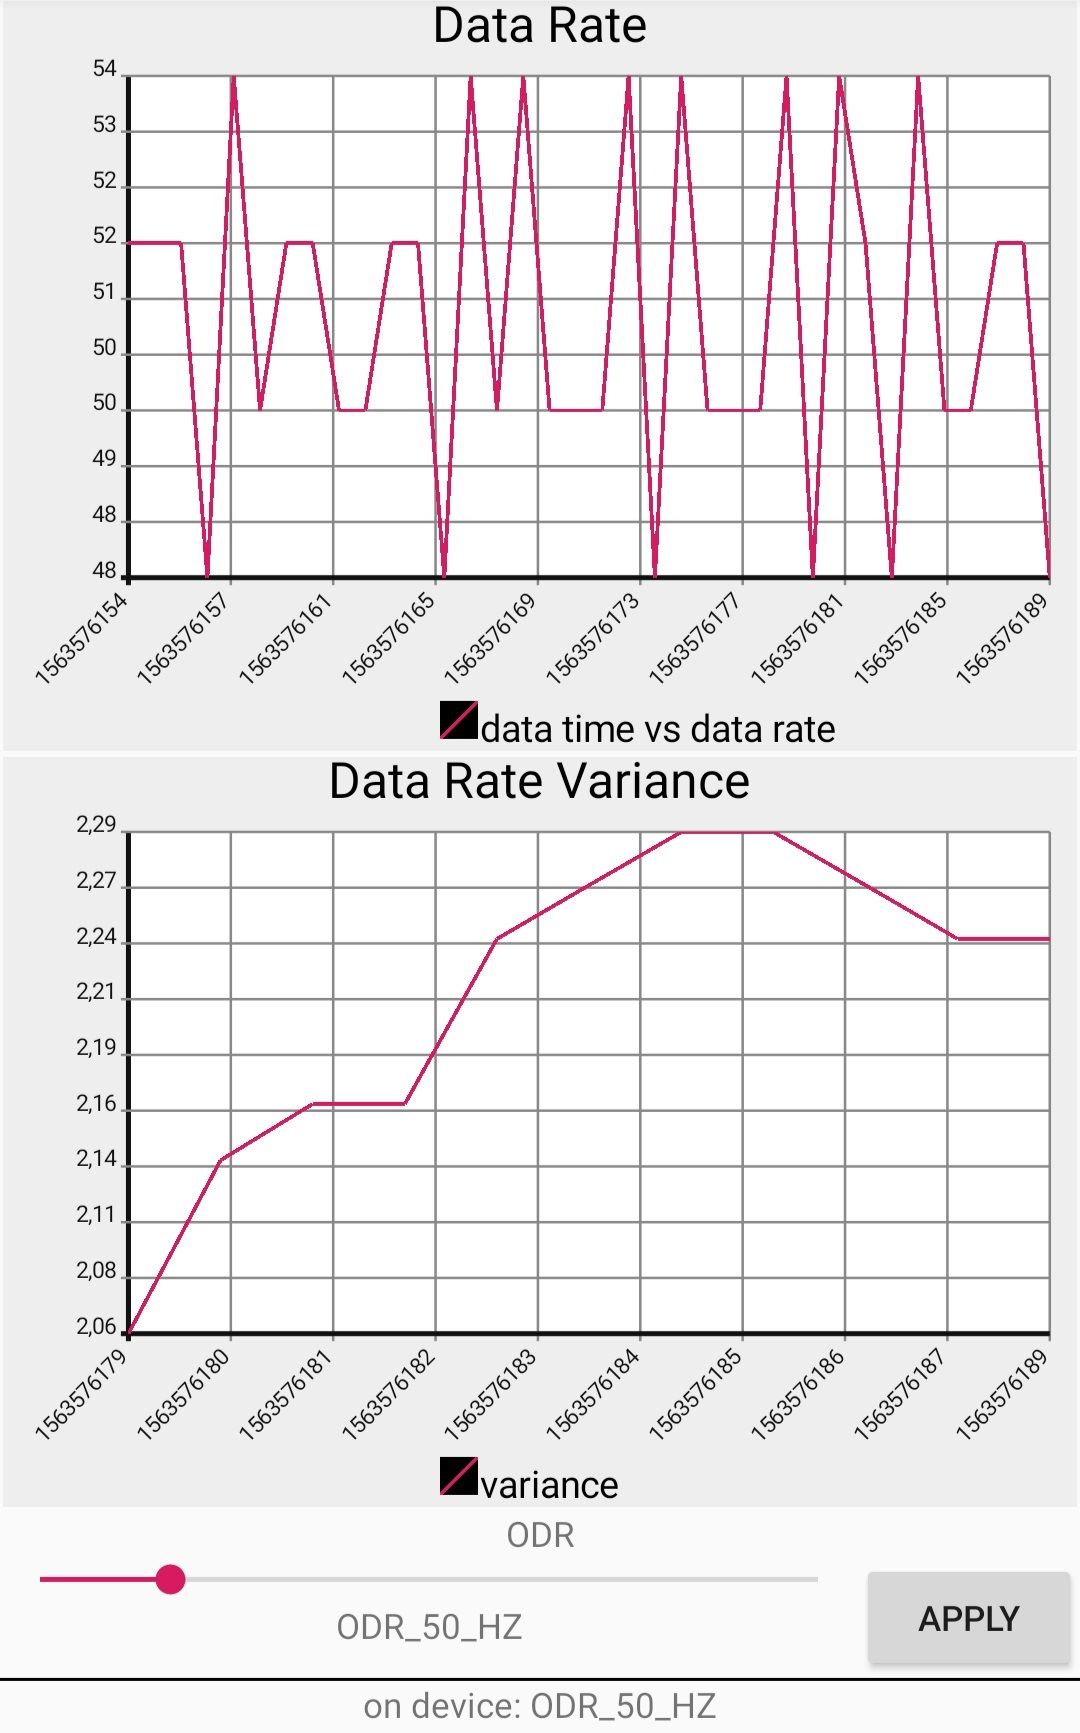
\includegraphics[width=0.5\linewidth]{res/android.jpg}
	\caption{Screenshot der Graphen von Datenrate und Standardabweichung}
	\label{fig:android}
\end{figure}
Um die Stromaufnahme zu messen, wird das ohmsche Gesetz $I = \cfrac{U}{R}$ benötigt.
Wird ein Widerstand in Reihe mit der Spannungsversorgung des Wearables geschaltet, ist ein Spannungsabfall um den Widerstand zu messen.
Da man den Wert des Widerstandes kennt und den Spannungsabfall mit einem Oszilloskop messen kann, lässt sich mit der Formel der Strom berechnen.
Bei der Wahl des Widerstandes gilt: Je größer der Widerstand, desto mehr Spannung fällt ab.
Ist die Spannung zu klein, lässt sie sich nicht genau messen.
Ist die Spannung zu groß, bleibt nicht genug Spannung für das Wearable übrig.
Um den Strom in verschiedenen Messbereichen berechnen zu können, werden die passenden Widerstände benötigt.
Zu Beginn der Evaluation wurde eine neue Batterie angebrochen, sodass etwa 3 Volt bereit stehen.
Da die MCU und IMU mindestens 1.71 Volt brauchen, werden die Widerstände so gewählt, dass der maximale Spannungsabfall weniger als 700 mV beträgt, damit die Funktionsfähigkeit gewährleistet bleibt.\\
Um den Widerstand anpassen zu können, wurde eine Lochrasterplatine, die in Abbildung \ref{fig:messplatine} zu sehen ist, mit Widerständen bestückt, die mit Steckbrücken in den Stromkreis integriert werden können.
\begin{figure}[hbtp]
	\centering
	\includegraphics[width=0.45\linewidth]{res/messplatine.jpg}
	\caption{Messplatine}
	\label{fig:messplatine}
\end{figure}
Die Widerstände haben eine Toleranz von 0.1 \% und Werte von 0, 10, 47, 100, 470, 1000, 4700 und 10000 Ohm.
Die Spannungsquelle ist eine CR2450 Knopfzelle.
Das Oszilloskop ist ein Picoscope 5444B.
Vor jedem Test wurde die Spannung der Batterie gemessen und das Offset des Oszilloskop kalibriert.
Der Spannungsabfall wurde mit einer Frequenz 2 GHz gemessen.
Technisch bedingt kann der Mittelwert nur über 5 Sekunden gebildet werden.
Deshalb wurde jeder Test 6 Mal abgeschlossen.

\section{Ergebnisse}
\subsubsection{Energieaufnahme mit LSM6DSL: Prototyp vs Wearable}
\subsubsection{Energieaufnahme auf Prototyp: LSM6DSL vs BMI160}
\subsubsection{Änderung von TX-Buffer}
\subsubsection{Änderung von MTU-Größe}
\subsubsection{Änderung von SPI-Frequenz}
\subsubsection{Änderung von Connection Interval}
\subsubsection{Änderung von Sensordatenrate}

\section{Analysis of Results}
